\chapter[Password Selection and the Decoy Effect]{Password Selection and the Decoy Effect}\label{chap:decoy}
%TODO: complete storyline from previous chapter (requirements elicitation)
	% thought: explicit need - suggestions, latent need: in an unexpected way, straightforward: you can see into the future if you adapt one of the suggestions; empower: make an informed decisions; --> there are a lot of points that we can pick up. 
	% but let's wait until we have feedback from judith
As laid out in Part \ref{part:problem_space}, one dimension of the problem space is that users pick weak passwords. In many situations, e.g. for unimportant accounts, this is acceptable. However, with rising importance, the need for a stronger password becomes salient. In these situations, mental models of password strength (see Chapter \ref{chap:pasdjo}) play a vital role, because they influence the choice of the password. There is increasing evidence that mental models are often sub-par: many users overestimate the strength increase from adding digits and symbols, or substituting letters with them \cite{Seitz2017PASDJO, Ur2015PWCreationLab, Ur2016PerceptionsPassword}. Thus, our goal is to avoid risky situations originating from flawed mental models. In this research project, we try to steer users away from weak passwords by providing more secure alternatives. Since it is hard to compete against a user's preferred password choice, we try to leverage persuasive strategies from marketing to ``sell'' the stronger alternative. This strategy is the so-called decoy effect. Given a range of products, vendors use this tool to make the one item stand out that is best for them (and often for the client). A decoy choice architecture includes one item that is ``unattractive by design'' to make a superior option salient. In numerous studies, it successfully shifted prospective buyers' reference point and achieved the goal. Thus, we aimed to translate it to the decision-making problem of selecting passwords. In essence, we can craft password suggestions in such a way that one of the suggestions is more attractive as judged by its strength and usability benefits. 

We thus aimed to answer the following research questions:

\begin{itemize}
	\item[\textbf{1)}] How can we translate the decoy choice architecture to password selection?	
	\item[\textbf{2)}] Does the decoy effect make users select stronger passwords?
	\item[\textbf{3)}] What are the opportunities and pitfalls in this approach?
\end{itemize}
	
To that end, we conducted an online experiment where different groups of participants received specific password suggestions. This chapter reports on the design and evaluation of a novel persuasive strategy and discusses the implications for its future application areas. Beside myself, Stefanie Meitner, Emanuel von Zezschwitz, and Heinrich Hussmann contributed to the project, which was first published at EuroUSEC 2016 \cite{Seitz2016DecoyEffect}.

% Motivation
% users use weak passwords 
% users think l33t speak is more secure than other strategies (pasdjo finding)
% but this is not necessarily the case, passphrases might be a better alternative
% hard challenge: mental model of passphrases indicates users think they are too weak. 
% RQ: how can this be changed?
% RQ: reverse misconceptions with ``marketing'' \cite{Ashenden2013SecurityLikeSoap}
% RQ: in which way do suggestions influence self-selected passwords?


\section{Background and Context}
Our project is positioned in a line of work that tries to nudge users towards strong passwords (see Section \ref{sec:rw:persuasive-interventions}). We approach this problem through two main components: suggestions and choice architecture. We briefly provide context on these two elements.  
%Goal: influence / correct mental models of password strength, persuade users to consider alternative strategies. 

%Criticism: this is unrealistic because memory interference effects prevent that this works for more than one account. -- yes, but for important accounts, this might still be worthwhile and people can more easily write down three words instead of an 8 character random sequence that might include ambiguous characters (0 and O); Kuo et al also say that writing down is a perfectly valid strategy \cite{Kuo2006HumanSelectionMnemonic}. (\todo{look up more researchers who argue in favor of writign down, e.g \cite{Kothari2017PasswordLogbooks} })

\subsection{Suggestions}
Suggesting passwords was at the heart of the first work on persuasion for stronger passwords \cite{Forget2008ImprovingPasswordsThroughPersuasion}. We can identify three common patterns here: (I) trying to get users to accept a suggested password verbatim\cite{Vance2013FearAppeals}; (II) suggesting alterations or insertions based on their own password \cite{Forget2008ImprovingPasswordsThroughPersuasion,Segreti2017AdaptivePolicies, Shay2015SpoonfulOfSugar}; or (III) suggesting a random password that serves as a basis for the user's password \cite{Huha2015UserReplaceablePasswords}. All password generators fall into the first category, because they encourage users to make sure the string is completely random. The second approach is the most common and most evaluated of the three, and has seen mixed results overall. Approach (III) seems promising in environments with critical security levels requiring more stringent policies. Moreover, suggestions are typically included real-time feedback where they can act as feed-\textit{forward} (opposed to feed\textit{back}) \cite{Ur2017DataDrivenPWMeter}. In summary, suggestions are an essential part of the persuasive toolkit and offer a wide range of new design opportunities.

\subsection{The Decoy Effect}
The decoy effect was discovered through research in consumer psychology. Buying a product usually involves deciding between different alternatives. On a high level, products are easily comparable by their quality and price, so customers heavily rely on these two metrics. The two dimensions also build the foundation of the decoy effect. In one of the first experiments on ``asymmetric dominance'', Huber \etal illustrate decision-making processes with a simple example to decide between six-packs of beer that differ in price and quality \cite{Huber1982AsymetricallyDominated} (slightly adapted for simplicity): 
\begin{table}[!h]
\begin{tabular}{lrr}
	\textbf{Option} & \textbf{Price} & \textbf{Quality rating}\\
	(A) & \$4 & 50 \small{/100}\\
	(B) & \$6 & 70 \small{/100}\\
\end{tabular}
\end{table}

While option (A) is cheaper than (B), it is also lower in quality. Spending \$2 more, the buyer will get a higher-quality beer (B). With the information available at this point, it is hard to decide. 
Buyers may have a general preference for either lower price, or higher quality if all other factors are excluded. Imagine the vendor wants to sell more of beer (A) because margins are higher for that product. To achieve this, Huber \etal explored different ways of adding a third option:
\begin{table}[!h]
\begin{tabular}{lrr}
	\textbf{Option} & \textbf{Price} & \textbf{Quality rating}\\
	(A) & \$4 & 50 \small{/100} \\
	(B) & \$6 & 70 \small{/100}\\
	(C) & \$4 & 40 \small{/100} \\
\end{tabular} 
\end{table}

Product (C) is as expensive as (A), but falls behind in quality. Thus, buyers will make a ``better deal'' if they choose option (A) by comparison with (C). Options (B) and (C) are more difficult to compare, because both dimensions (price and quality) are higher in (B) and make it appear like an outlier. Option (C) is thus called the \textbf{decoy} that is \textit{dominated} by option (A) (\textbf{target}). Option (B) (the \textbf{competitor}) also beats the decoy, but the comparability between the target and the decoy boosts the favorability of the target. This is exactly what Huber \etal found, and which was later confirmed numerous times in different decision-making scenarios \cite{Ariely1995ExplanationSubjectiveDominance}. Adding the decoy has the potential to reverse existing preferences, making it a powerful tool for marketing and sales. The decoy itself often serves the sole purpose of making another item stand out, thus the underlying persuasion principles are \textbf{salience} and \textbf{framing}. Constructing the dimensions in a certain way is referred to as \textit{choice architecture} \cite{Thaler2010ChoiceArchitecture}, and is an important persuasive design strategy. 

Huber \etal stated that there is a specific combination of attributes to position the decoy (see Figure \ref{fig:decoy:general-construction}). Depending on the target, the decoy acts as range increasing (R, R*), frequency increasing (F), or both (RF). By extending the range on the dimension on which the \textit{competitor} is superior, the fixed difference between all items on that dimension is weighed less. Figure \ref{fig:decoy:beer-construction} illustrates this type of decoy placement for the sixpack example. The range of the quality is clearer after the decoy is added: before the span was [50;70], and afterwards [40;70]. The superiority of the competitor appears less significant, hence the higher price can seem unjustified. 

%- decoy: vendor does not intend to sell this, it acts as an unfavorable alternative that can be used as reference point / comparison.\\	

\begin{figure}[t]
	\centering
	\begin{subfigure}[t]{0.49\textwidth}
		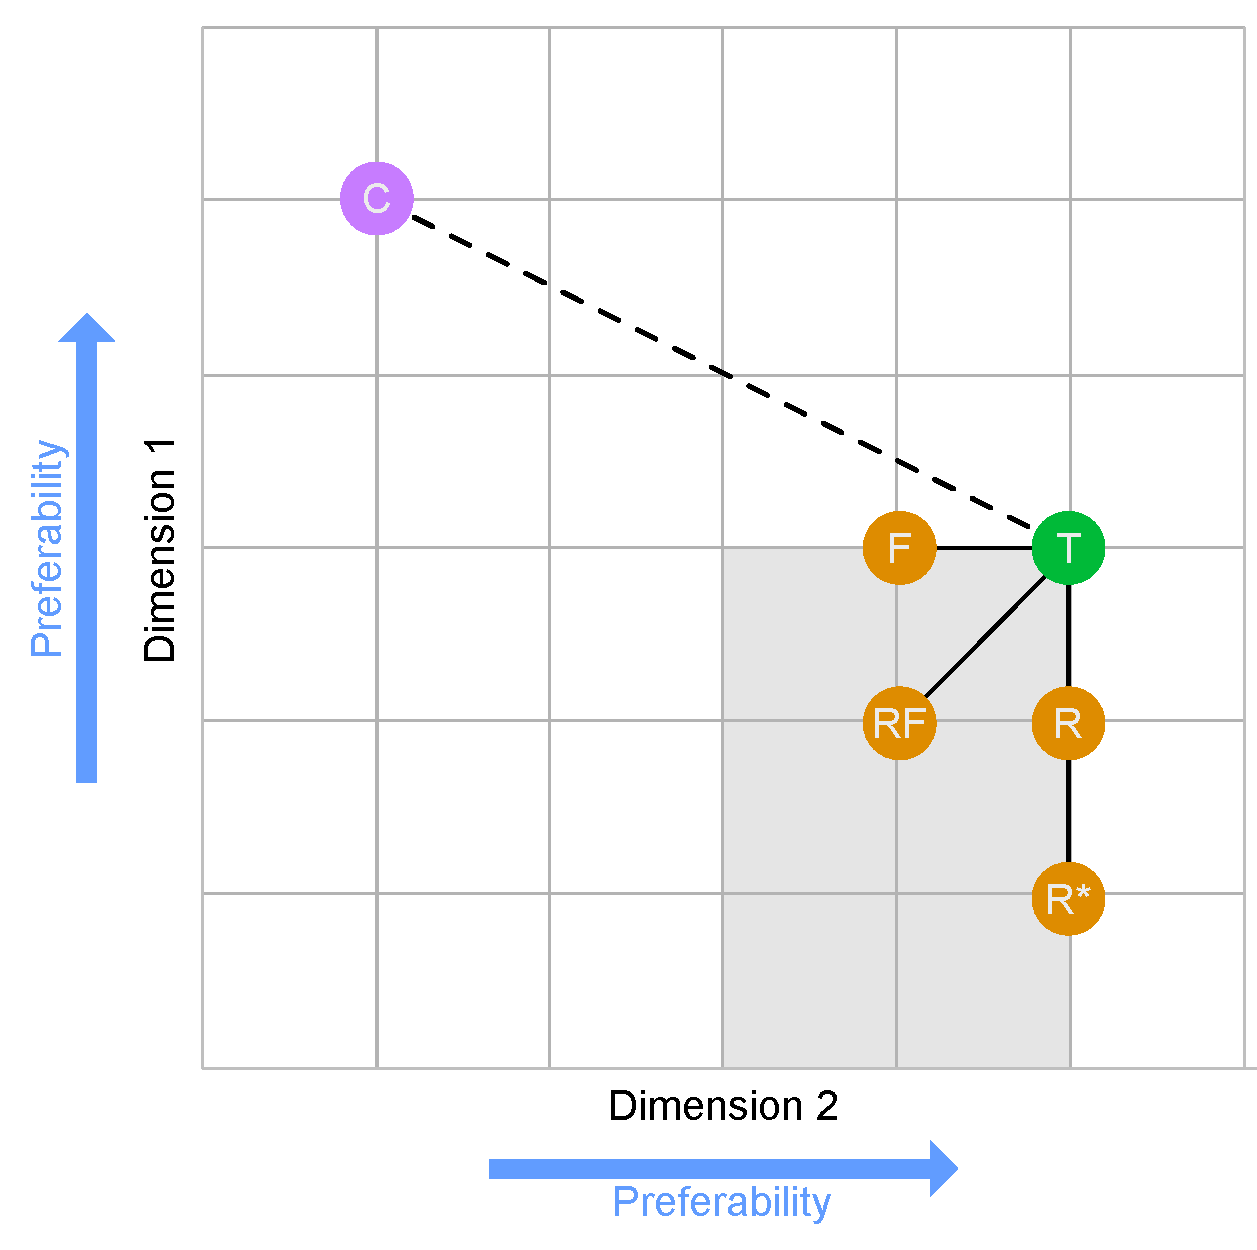
\includegraphics[width=\textwidth]{figures/decoy/decoy-dimensions-general}
		\caption{\label{fig:decoy:general-construction}Decoy placement options \cite{Huber1982AsymetricallyDominated}}
		
	\end{subfigure}
	\begin{subfigure}[t]{0.49\textwidth}
		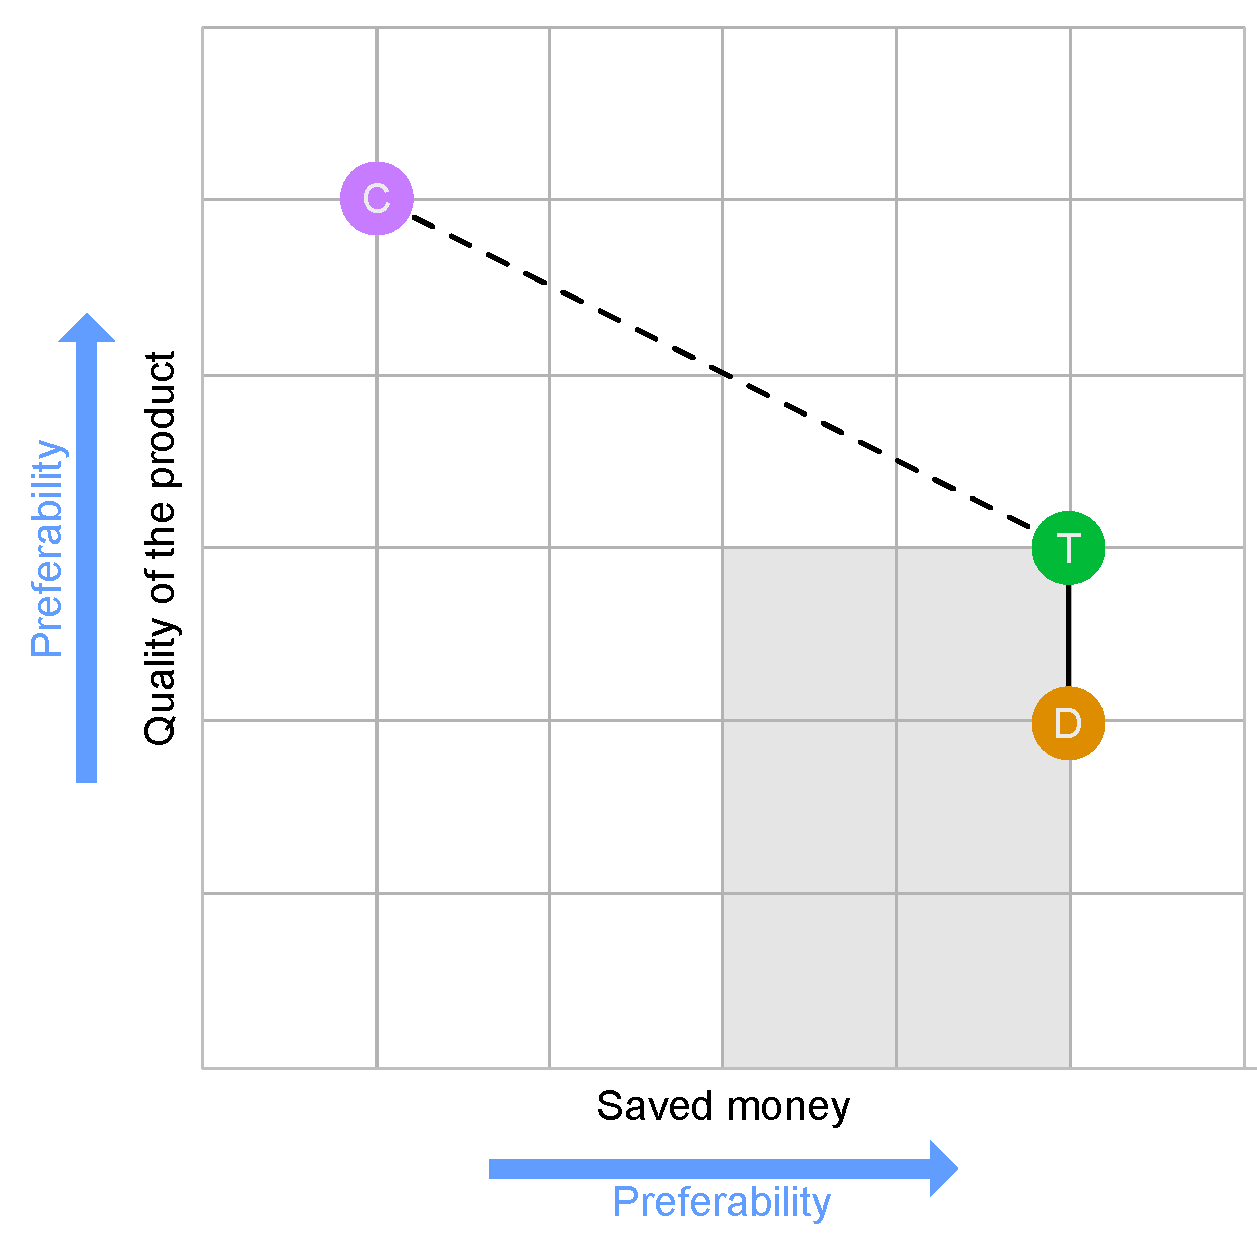
\includegraphics[width=\textwidth]{figures/decoy/decoy-dimensions-beer}
		\caption{Example choice architecture for sixpack of beers.}
		\label{fig:decoy:beer-construction} 
	\end{subfigure}
	\caption{
		General choice architecture overview to generate asymmetric dominance. 
		C = competitor, T = Target. The decoy can be placed at different positions in the spectrum, but needs to be dominated by the target (gray areay). Placement strategies for the decoy to increase the target's dominance: R = Range, R* = extreme range, F = frequency, RF = range and frequency.
	} 
\end{figure}

%- broader concept: framing, salience, anchoring. 
%- making choices, given a set of alternatives
%- using a decoy choice architecture to influence the preferred option 

\subsubsection{Example: Decoy Effects in the Real World}
Huber \etal's example has been adapted and used in the design of user interfaces. The vendor, i.e. a service provider, tries to steer users towards a particular direction that they see as favorable. For instance, location settings on an Android device show signs of a decoy pattern (see Figure \ref{fig:decoy:android-pattern}). From bottom to top, the ``device only'' mode activates the GPS module to determine the device's location. It is thus highly accurate outside of buildings, but does not work well inside. On the other hand, the ``battery saving mode'' works in both environments by using Google's online location services based on triangulation between network cells and surrounding WiFis. In urban areas and even inside buildings, it can achieve great accuracy, while it only roughly estimates locations in rural areas. The two accuracy-levels are thus comparable, but the ``battery saving mode'' does not require powering up additional antennae and modules, giving it a graspable advantage. The ``High accuracy'' mode combines both approaches and is thus the most battery consuming, but most versatile option. The ``battery saving'' can be seen as the target, because it provides the best trade-off in most situations. The ``device only'' mode is the decoy because it uses more battery, while the ``high accuracy'' mode is the competitor. Google requires the user to allow the collection of technical sensor data for the ``high accuracy'' and ``battery saving'' mode. Battery consumption is likely more important to users than location accuracy, which further suggests that the ``battery saving'' mode is indeed the targeted setting. 

\begin{figure}
	\centering
	\begin{subfigure}[!t]{0.49\textwidth}
		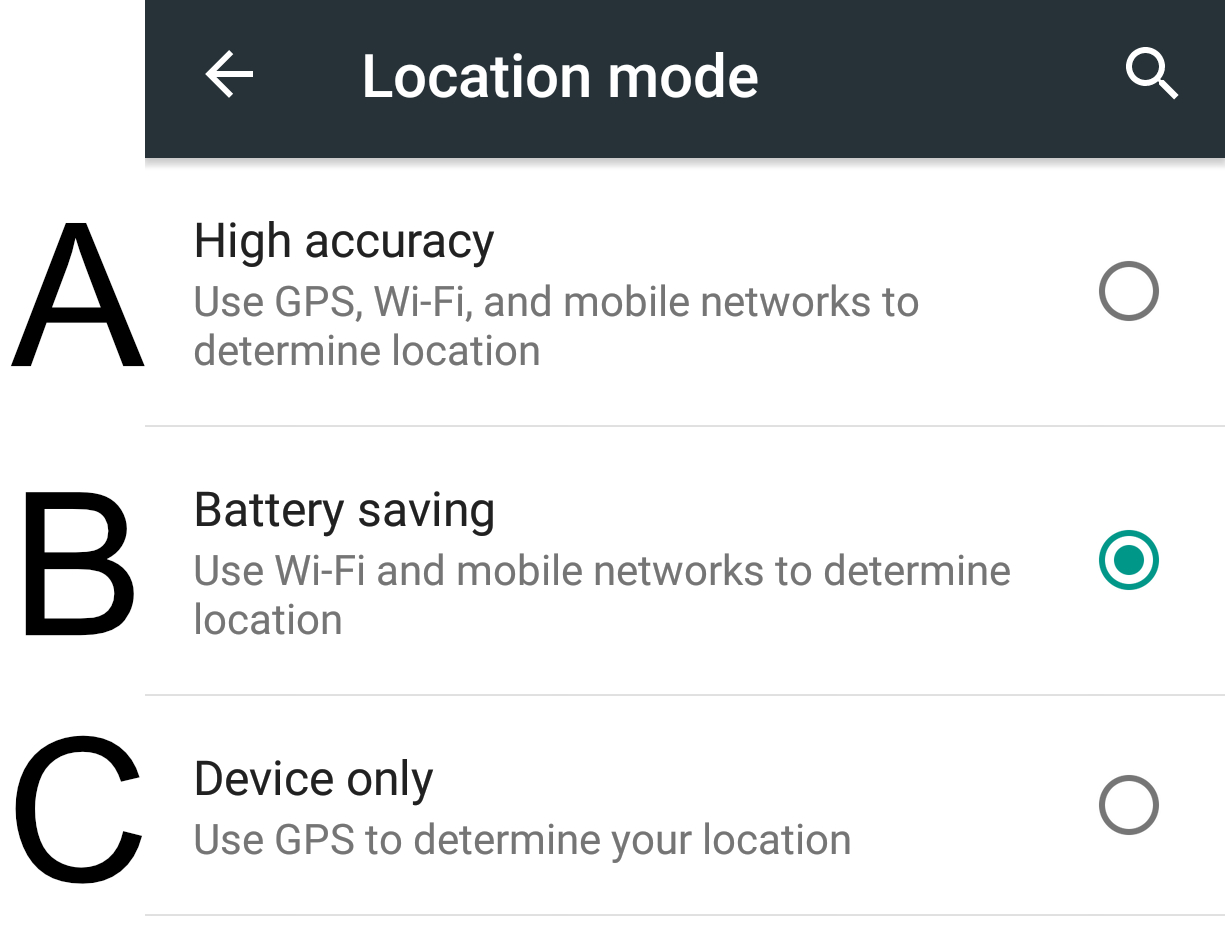
\includegraphics[width=\textwidth]{figures/decoy/Android_Location_Decoy}
	\end{subfigure}
	\begin{subfigure}[!t]{0.49\textwidth}
		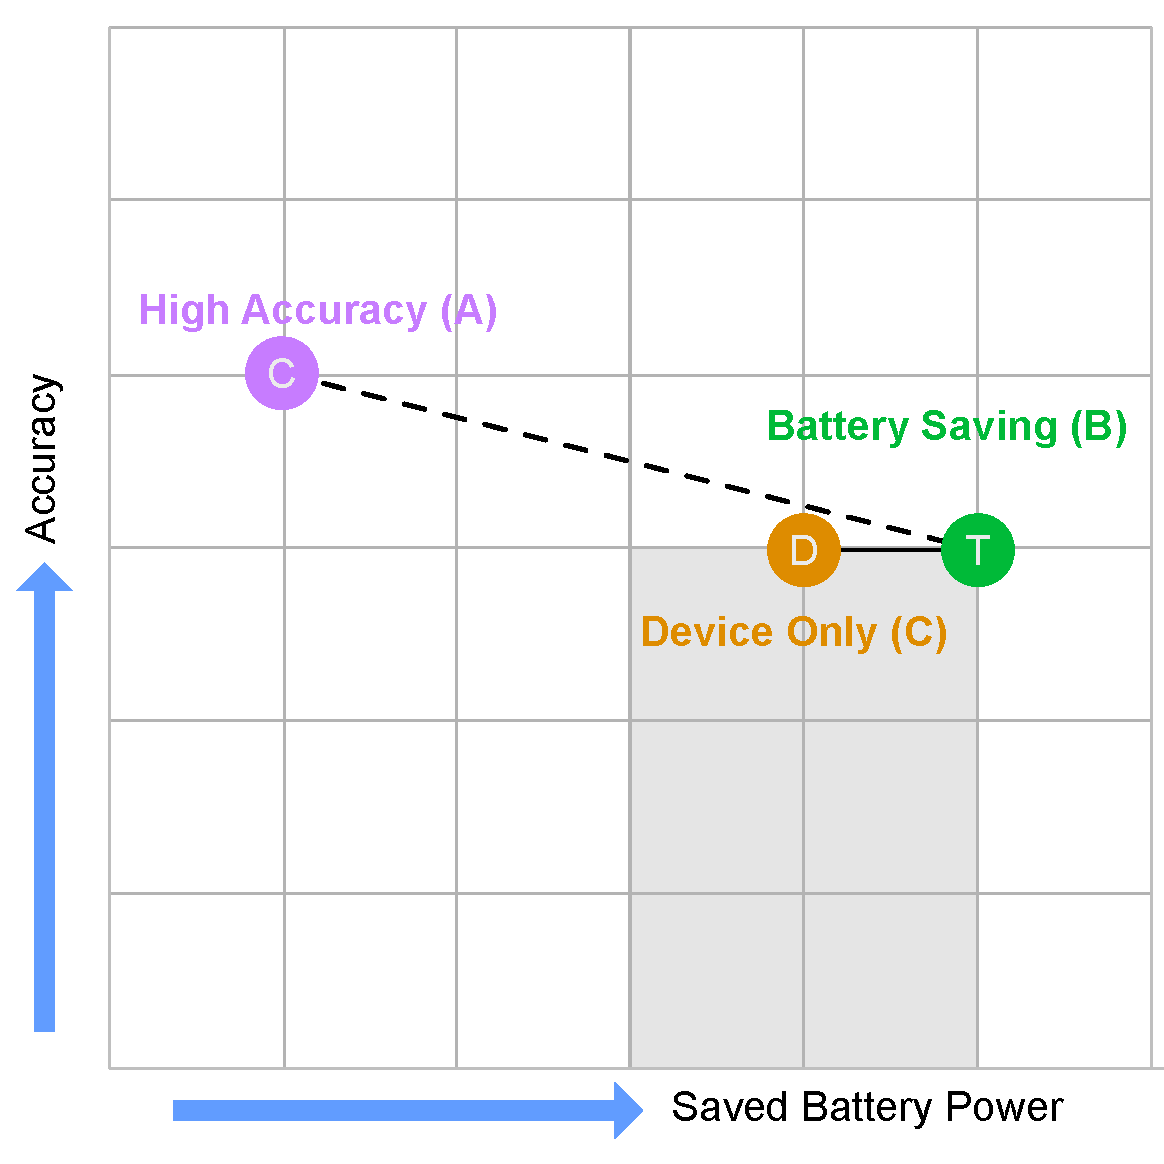
\includegraphics[width=\textwidth]{figures/decoy/decoy-dimensions-android}
	\end{subfigure}
	\caption{\label{fig:decoy:android-pattern}Location settings in Android show signs of a decoy pattern. The ``battery saving'' mode is targeted, because it does not activate the GPS module and can achieve comparable accuracy. Google benefits from collecting information on WiFi hotspots and network cells to improve their location service.} 
\end{figure}


\subsection{Choice Architecture in Security and Privacy}
The \gls{USEC} community has started to investigate the feasibility of behavioral economics principles in the design of security and privacy mitigations. Egelman \etal showed that choice architecture is highly relevant for privacy settings on mobile devices \cite{Egelman2013ChoiceArchitecture}. They explored how users value privacy-respecting apps and how they make decisions from a list of applications. To measure preferences, they put monetary values and discounts on permissions like accessing the Internet or using device location. Participants in their study showed clear decision-making patterns that were influenced by the price and type of permission. Therefore, Egelman \etal concluded that a certain choice architecture can guide users towards a more ``rational behavior''. 

Knijnenburg \etal \cite{Knijnenburg2013MorePrivacyOptions} explored the \textit{choice proliferation} phenomenon in location-privacy settings. The principle indicates that people become choice averse with an increasing number of options. In their study, they observed that participants were strongly influenced by the number of available options to share their location. Without specifically mentioning it, they also used a \textit{decoy} option that was extremely unfavorable, but triggered a change in preference. In another study, Korff and Böhme showed that the granularity of privacy settings on a business social network can have similar effects: participants in their study tended to stick with default settings and were also less satisfied with their choices \cite{Korff2014TooMuchChoice}. Acquisiti \etal showed that such architectures can nudge users towards certain settings \cite{Acquisti2017NudgesPrivacySecurity}. 

Regarding passwords, only few publications mention the use of choice architectures. Renaud \etal evaluated a wide range of nudges to make users of a university platform pick a stronger passwords. They concluded that the tested architectures were fairly ineffective in achieving this goal, but there might have been other more effective solutions beyond their designs. Before our own investigation, no study that we are aware of has explored the decoy paradigm for passwords. 

% might be mentioned briefly:%
%\cite{Wang2014PrivacyNudgesFacebook}
%\cite{Malkin2017PersoanlizedSecurityMessaging}
%\cite{Jameson2011PreferentialChoice}

\section{Designing Password Choice Architecture}
% Briefly point to first exploration report to mention a design that failed. 
We aimed to craft a nudge that persuades users to create stronger passwords. Respecting the principle of the opportune moment, we opted for account creation contexts. To emulate a situation that is comparable to buying one out of several product alternatives, we show suggestions beneath the password field where the user enters their choice (see Figure \ref{fig:decoy:design-architecture-prolific}). We ended up with this design after identifying opportunities of strength feedback on the user's password and on the suggestions (i.e. feed-forward). To that end, we had created several prototypical choice architectures and rapidly evaluated them in the lab and online (see technical report \cite{Seitz2016DecoyEffectReport}). The final architecture implements the propositions in Huber \etal's framework (see Figure \ref{fig:decoy:dimensions-prolific}).

\begin{figure}[t]
	\centering
	\begin{subfigure}[!t]{0.49\textwidth}
		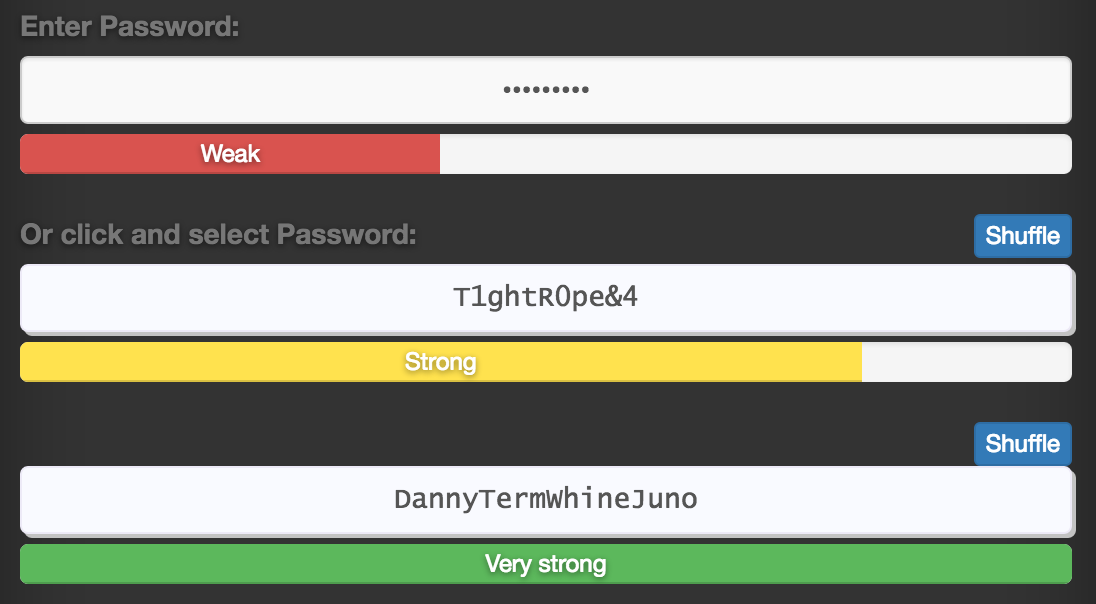
\includegraphics[width=\textwidth]{figures/decoy/generator_prolific_3}
		\caption{\label{fig:decoy:screenshot-prolific}}
	\end{subfigure}
	\begin{subfigure}[!t]{0.49\textwidth}
		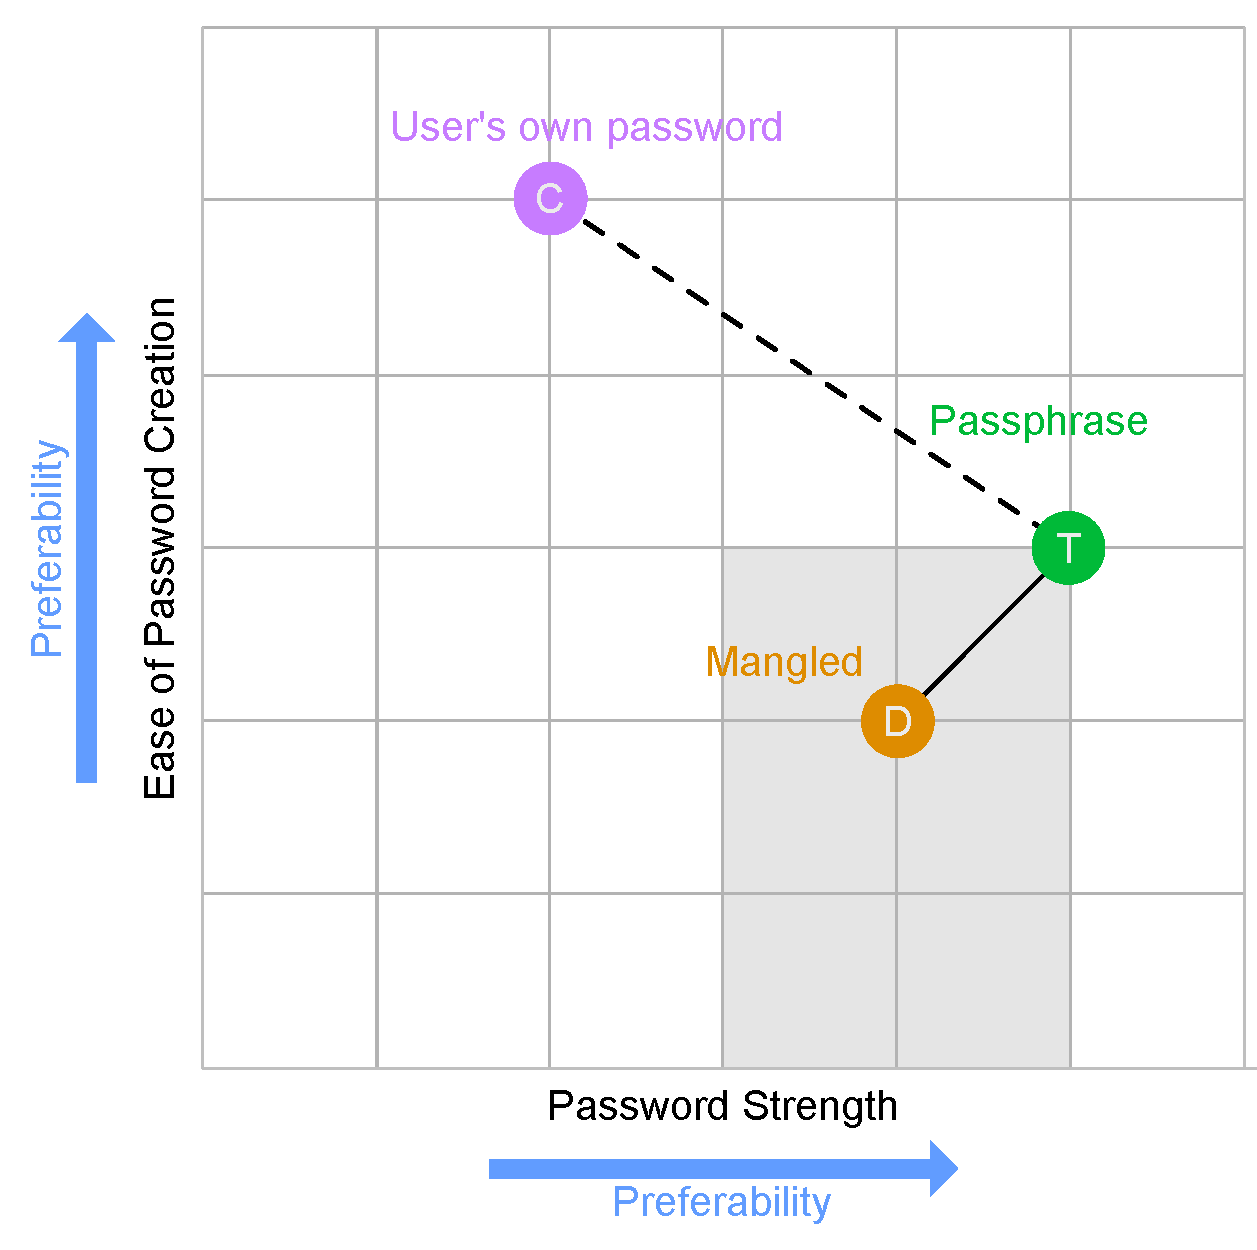
\includegraphics[width=\textwidth]{figures/decoy/decoy-dimensions-prolific}
		\caption{\label{fig:decoy:dimensions-prolific}}
	\end{subfigure}
	\caption{\label{fig:decoy:design-architecture-prolific}Choice architecture and decoy placement as evaluated in the online experiment. } 
\end{figure}

The key to password choice architecture is the user's own password. It has to be seen as the \textbf{competitor}. Service providers will want accept the user's own password, because they want make sure users sign up. On the other hand, they want to avoid attacks on user accounts, which is why they likely encourage using a stronger password. This is the \textbf{target}. In our design, we opted for a \textit{passphrase} as target for several reasons: only few users create secure passphrases as their primary credentials \cite{Ur2015PWCreationLab}; passphrases provide usability and memorability benefits \cite{Keith2009PassphraseDesign}; self-selected passphrases often do not provide the desired security benefits \cite{Bonneau2012LinguisticProperties}, which can be mitigated by supplying users with a combination of random words \cite{Shay2012CorrectHorseBatteryStaple}. 

To make the passphrase preferable over the competitor, a decoy needs to be carefully positioned along the two dimensions such that it is closer to the target than to the competitor. Moreover, it needs to be dominated at least in one dimension by the target. To achieve this, we identified ``ease of use'' and ``security benefits'' as two feasible dimensions of the choice architecture. We opted for a range-frequency decoy (see Figure \ref{fig:decoy:general-construction}) where the target dominates the decoy in \textit{both} dimensions, because effects are more likely to be detected this way. A typical-length \textit{mangled} password fulfills the criteria. The richer character set includes symbols that require the Shift/Alt keys to enter them. Thus, the ease of creation is lower than that of a passphrase (dimension 1). At the same time, typical mangling strategies only slightly contribute to password strength, which we confirmed in Chapter \cite{chap:pasdjo}. Passphrases are considered stronger by several estimators. Consequently, mangled passwords are dominated by passphrases regarding strength (dimension 2). Figure \ref{fig:decoy:dimensions-prolific} illustrates the positioning along the two dimensions.

\section{Quantitative Evaluation}
We ran an online experiment to evaluate the efficacy of our decoy choice architecture for passwords. We formed the following hypotheses about the outcome:
\begin{description}
	\item[H0] Participants' self-selected passwords are comparable in strength and memorability, regardless of the presence of a password suggestion (Nullhypothesis). 
	\item[H1] The presence of a single password suggestion will lead to slightly stronger passwords.
	\item[H2] The presence of two suggested passwords that follow a decoy choice architecture regarding strength and ease of use will lead to stronger passwords that resemble the target suggestion. 
\end{description}

\subsection{Method}
% study design, independent variable
The study implemented a between groups design. The main task was creating a new password under one of four treatments. ``Suggestion architecture'' served as independent variable with three levels: \textbf{Passphrase}, \textbf{Mangled}, and \textbf{Decoy}. Each level was tested with a separate participant group. In the Passphrase condition, participants were suggested a single passphrase consisting of four words. Analogously, a higher-complexity password is displayed in the Mangled condition. The Decoy group received both the target passphrase and the complex decoy password as alternative suggestions to their own password. Having study conditions with single suggestions allowed us to measure the impact of the decoy effect. All suggestions are accompanied by visual and textual representations of zxcvbn scores. The labels for the different strength scores were \textit{very weak, weak, ok, strong, very strong}. To obtain a baseline for comparison, there were no password suggestions for the \textbf{Control} group. However, participants in this group received strength feedback allowing us investigate the impact of suggestions. 

%dependent variables
We did not collect plain text passwords to ethically deal with participants disclosing their real passwords. Instead, we used modified the zxcvbn library by stripping all sensitive information\footurl{https://gist.github.com/TobiasSeitz/e27a867535b82f6cf9a6ae6140da8b81}{06.03.2018}, and analyzed participants' passwords on the fly. These \textit{meta statistics} served as dependent variables and were saved to a regular database. Most notably, they describe the password topology (length, number of upper-/lowercase, digits, symbols, and chunks), estimated guess numbers and the zxcvbn score. Scores range from 0 (weak) to 4 (strong), while guess number estimates are open-end. Another dependent variable was memorability which was measured by a successful authentication three days after password selection. To achieve this, we hashed passwords with a secure one-way function (PHP's \texttt{password\_hash()}) and compared hashes afterwards. If they matched, the password was correct, thus this is a binary metric.

\subsubsection{Prototype}
For the purpose of the study, we implemented the concept as web-prototype based on HTML and JavaScript. As foundation for the generating passwords in all conditions, we relied on the Diceware dictionary\footurl{http://world.std.com/\~reinhold/diceware.wordlist.asc}{06.03.2018} consisting of 5823 words. It provides a good spectrum of common and uncommon words of varying length. To generate the passphrase (target), four words were randomly combined and capitalized individual words. As shown in Chapter \ref{chap:pasdjo} zxcbvn rates four-word passwords with its highest score. The randomness of generated passwords allows us to calculate their entropy. Each word has an estimated entropy of $(log_2(5823) \approx 12$ bits. Combining four words randomly thus results in a total entropy of approximately $ (2^{12})^4 = 48$ bits for passphrases.

For the decoy and the mangled password condition, the prototype modifies a randomly selected word from a smaller subset of the Diceware list. The subset only includes words longer than eight characters, giving a total of 687 candidates. The first letter of the word, and a second randomly chosen character are capitalized. Two letters are substituted by similarly-looking digits to inspire a \textit{l33t} character. For instance, the letter ``o'' was replaced with the digit ``0''. Finally, a random symbol and digit are appended to the word. The resulting decoy password consists of four different character classes (LUDS). 

We anticipated that the generated passwords are exceptionally unattractive in some cases, e.g. if passphrases consist include uncommon, hardly memorable words, e.g. \texttt{GirthInflixThineAegis}. To make them more appealing, the prototype provides a \textit{shuffle} button that gives a new combination of words (see Figure \ref{fig:decoy:screenshot-prolific}). The mangled password can also be re-generated. Another feature to lower barriers to take one of the suggested passwords was the opportunity to transfer it to the password field with a single click. However, to facilitate memorization, participants needed to manually type the password into the confirmation field. 

\subsubsection{Procedure}
The experiment consisted of two parts that were carried out on separate days. The initial step included the password selection task and usability assessment among other qualitative metrics. Participants were invited to return for the second part of the study three days later. This follow-up step included memorability assessment and further qualitative feedback to help us understand the data.

The first part started with a thorough briefing about the collected data and asked for consent. The same web-page introduced the scenario for the task: Participants were asked to imagine creating a new password for their already existing email account under a basic8 policy. The page displayed the password fields and suggestions. Participants were randomly assigned to one of the four treatment groups, so the type and number of suggestions depended on this assignment. Once the password was successfully confirmed, participants were asked to fill out a brief questionnaire mostly consisting of 5-point scale items on attitudes and password behaviors. At the end of the first part, the web-page displayed a confirmation code that participants had to copy over to the prolific platform to mark the survey as done. 

Three days afterwards, we invited the participants to return and complete the second part. They were asked to provide the password they had remembered, but we did not validate 

\subsubsection{Recruitment and Sample}
Following best practices in password research, we leveraged crowd-sourcing tools to elicit the data. Recruitment took place through the research platform Prolific\footurl{https://prolific.ac}{06.03.2018}, which is comparable to Amazon's Mechanical Turk solution. Participants were screened for age (older than 18 years), and they had to be located in either the UK or in USA. The region restriction was introduced because Prolific has a larger user base in those countries. To ensure quality of the data, we required a past survey completion rate of at least 95\%. This is a common metric for the reliability of a crowd-worker \cite{Ross2010WhoAreTurkers}. 

From the 106 respondents who started the experiment, we had to reject seven because the study completion code was wrong or missing, or because the questionnaire was insufficiently filled out or completion times were outliers ($> 3*SD$). The remaining 99 participants received invitations to return, which 97 people did. There were another fourteen incomplete responses or wrong study codes. Hence, the resulting N of our data set is $N = 83$ valid, complete responses in both parts. Group sizes were $n=18$ in Control, $n=24$ in Passphrase, $n=21$ in Mangled, and $n=20$ in Decoy. On average, participants were 30 years old ($SD=10$). 42\% were female. The majority (78\%) was employed, 12\% were students, 10\% were unemployed. Participants reportedly possessed nine online accounts that they regularly use ($SD=5.6$). 

%no CS students: just like in \cite{Wash2016UnderstandingPasswordChoices}

%live deployment. 
%users could shuffle. 

\subsection{Results}
Through statistical tests we found significant differences across the groups. Although the decoy effect did not work as intended, there were notable side-effects. In the following, we break down the findings. For non-parametric continuous data, we used Kruskal-Wallis and Mann-Whitney tests, whereas frequencies were analyzed with chi-squared tests. Significance levels were set to $\alpha = 0.05$, unless multiple comparisons required a Bonferroni correction. 

\subsubsection{Efficacy of Suggestions} 
\begin{figure}
	\centering
	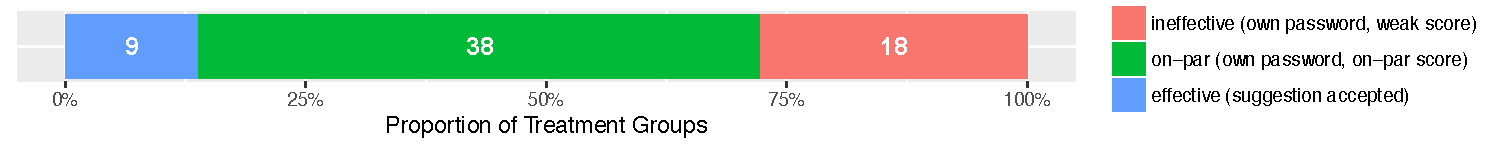
\includegraphics[width=\linewidth]{decoy/treatment-impact-edited}
	\caption{\label{fig:decoy:treatment-impact-edited} Nudge efficacy in treatment groups (n=65)}
\end{figure}
Across all treatment groups, nine respondents out of 65 ($\approx$ 14\%) accepted a suggested password verbatim -- four in the Passphrase group, two in the Mangled group, and three in the Decoy group (two targets, one decoy). Suggestions were thus effective for one in ten participants. From the remaining 56 self-selected passwords, 18 (27.7\%) were weaker than the suggestions. In other words, the nudge was ineffective for roughly a third of participants judged by their choice to pick a password that was weaker than the suggestion. For the remaining 38 participants (58.4\%), the nudge could have influenced them to create passwords that as strong as the suggestions, but we lack data to investigate this. Figure \ref{fig:decoy:treatment-impact-edited} visualizes the efficacy of suggesting passwords.

\subsubsection{Impact on Password Strength}
Table \ref{tbl:decoy:zxcvbn-m-sd} lists descriptive statistics on password strength metrics. Taking the entire sample into account, omnibus tests did not show significant differences between the four groups. However, we plotted the confidence intervals of all metrics to examine the data visually. Here, it is visible that guess numbers did notably differ between the groups: the Passphrase treatment led to the strongest passwords overall (see Figure \ref{fig:decoy:ci-guesses-all}). If we remove the samples where a suggestion was accepted, the differences become smaller (see Figure \ref{fig:decoy:ci-guesses-own}). Since guess numbers are shown on a logarithmic scale, the difference appears might appear smaller than it actually is: guess numbers in the passphrases group were about 50 times higher than in the control and mangled groups. This is also visible in Figure \ref{fig:decoy:guess-number-plot}, where the percentage of cracked passwords is consistently smaller than in the other groups. Fitting a smoothed generalized additive model to the cracked percentages confirms that passwords are less likely to be cracked after any given number of guesses, if they were created in the Passphrase condition ($intercept=Control,B=-7.9\%, p<0.001$. \Rsqadj{0.99}). The rise in strength most likely is due to increased password length in the Passphrase group, see Figure \ref{fig:decoy:ci-length-own}.

\begin{table}
  \centering
  \caption{\label{tbl:decoy:zxcvbn-m-sd}Summaries of password metrics from the online experiment. Arranged by group (columns) and metric (rows)}
    \begin{tabular}{p{2cm}rr|rr|rr|rr}
    \toprule
          & \multicolumn{2}{c}{\textbf{Control}} & \multicolumn{2}{c}{\textbf{Mangled}} & \multicolumn{2}{c}{\textbf{Passphrase}} & \multicolumn{2}{c}{\textbf{Decoy}} \\
    \midrule
          & \multicolumn{1}{c}{M} & \multicolumn{1}{c}{SD} & \multicolumn{1}{c}{M} & \multicolumn{1}{c}{SD} & \multicolumn{1}{c}{M} & \multicolumn{1}{c}{SD} & \multicolumn{1}{c}{M} & \multicolumn{1}{c}{SD} \\
    length & 11.33 & 3.53  & 11.8  & 2.74  & 13.87 & 3.8   & 11.9  & 2.69 \\ 
    score & 2.88  & 1.02  & 2.9   & 0.76  & 3.29  & 0.9   & 2.95  & 0.88 \\
    guesses$_{log10}$ & 8.84  & 2.41  & 8.86  & 2.15  & 13.48 & 7.63  & 10.12 & 4.85 \\
    digits & 2.61  & 2.06  & 2.28  & 1.27  & 2.16  & 2.18  & 2.6   & 2.34 \\
    special & 0.22  & 0.64  & 0.52  & 1.16  & 0.2   & 0.5   & 0.3   & 0.57 \\
    uppercase & 1.77  & 0.8   & 1.42  & 0.59  & 2.45  & 2.35  & 1.75  & 1.11 \\
    lowercase & 6.55  & 3.91  & 7.38  & 3.21  & 8.91  & 4.09  & 6.95  & 3.42 \\
    \bottomrule
    \end{tabular}%
\end{table}%

%None of the participants' passwords was scored as ``very weak'' (0). 

\begin{figure}
	\centering
	\begin{subfigure}[c]{0.45\textwidth}
		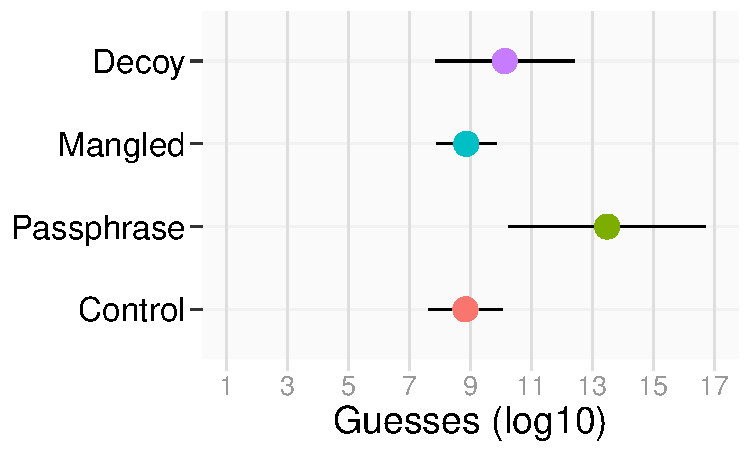
\includegraphics[width=\textwidth]{figures/decoy/ci-guessesLog10-all}
		\caption{\label{fig:decoy:ci-guesses-all} Confidence intervals of estimated guess-numbers (log 10) for all participants (N=83). On average, the Passphrase group created significantly stronger passwords than the Control and Mangled group.}
	\end{subfigure}
	\begin{subfigure}[c]{0.45\textwidth}
		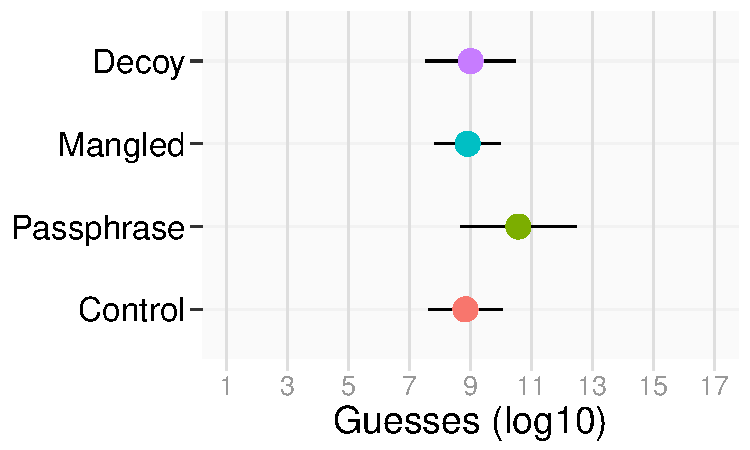
\includegraphics[width=\textwidth]{figures/decoy/ci-guessesLog10-own}
		\caption{\label{fig:decoy:ci-guesses-own}
			Confidence intervals of estimated guess-numbers (log 10) for self-selected passwords (N=74). Although the difference between the Passphrase group and the others is not as big as in the overall sample, the average guess numbers are still $\approx$ two orders of magnitude apart.}
	\end{subfigure}
	\caption{\label{fig:decoy:results-strenth} Arithmetic mean of guess numbers (log 10) and 95\% confidence intervals.} 
\end{figure}

\begin{figure}
	\centering
	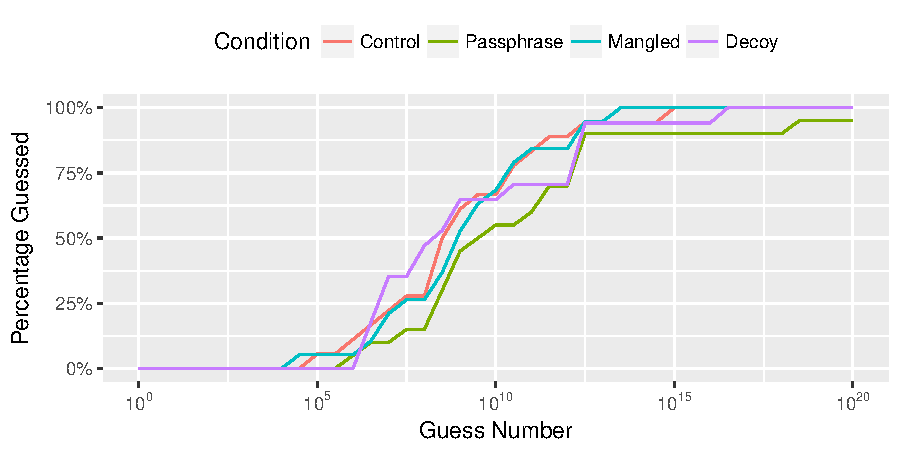
\includegraphics[width=0.8\linewidth]{decoy/guess-number-plot}
	\caption{\label{fig:decoy:guess-number-plot} Estimated guessability of user-selected passwords across the four conditions.}
\end{figure}

\begin{figure}
	\centering
	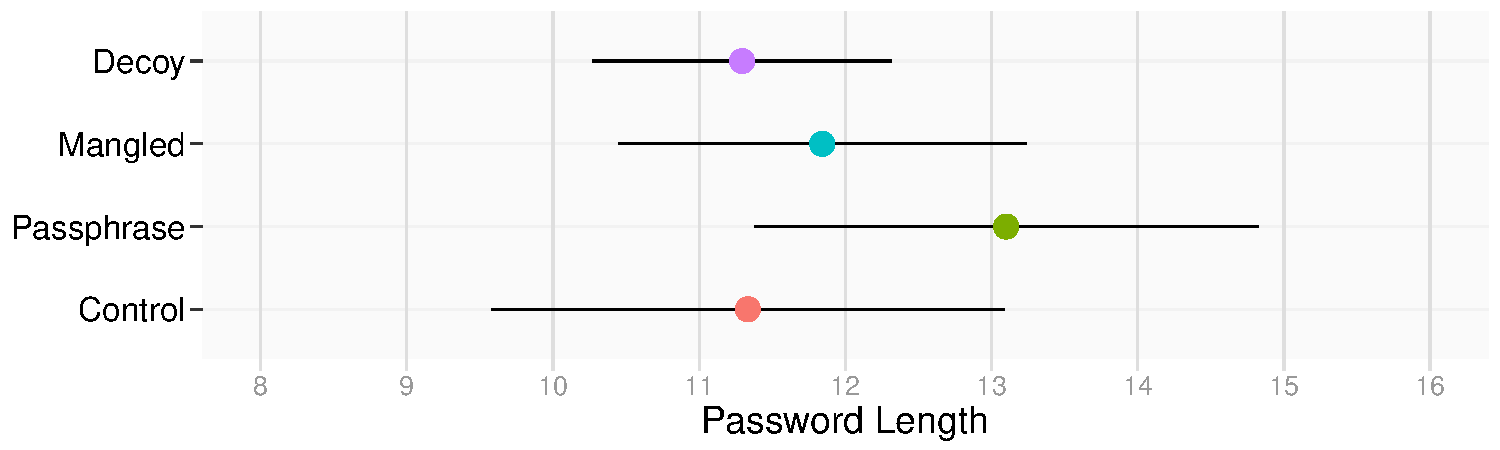
\includegraphics[width=0.8\linewidth]{decoy/ci-length-own}
	\caption{\label{fig:decoy:ci-length-own} Average password length of self-selected passwords and 95\% confidence intervals}
\end{figure}

%\subsection{Live-Deployment Data}
%Talk about a couple of findings of the Roskilde dataset. 
% nah. there's no time for that now. 
%TODO add screenshot from roskilde sign-up. 

\subsubsection{Password Composition and Policy Adherence}
\begin{table}
  \centering
  \caption{\label{tab:decoy:policies}Policy fulfillment of submitted passwords. Most participants used at least three character classes.}
    \begin{tabular}{rrrrrrrr}
    \toprule
          & \begin{turn}{45}comp8\end{turn} & \begin{turn}{45}3class8\end{turn} & \begin{turn}{45}3class12\end{turn} & \begin{turn}{45}3class16\end{turn} & \begin{turn}{45}basic8\end{turn} & \begin{turn}{45}basic12\end{turn} & \begin{turn}{45}basic16\end{turn} \\
    \midrule
    Control     & 2     & 9     & 4     & 0     & 1     & 1     & 1 \\
    Mangled    & 6     & 7     & 3     & 3     & 1     & 1     & 0 \\
   Passphrase   & 4     & 5     & 4     & 2     & 1     & 1     & 7 \\
    Decoy    & 5     & 7     & 3     & 1     & 1     & 1     & 2 \\
    \midrule
    $\Sigma$  & 17    & 28    & 14    & 6     & 4     & 4     & 10 \\
    \bottomrule
    \end{tabular}%
\end{table}%%tab:decoy:policies%
It is possible to sort participants' self selected passwords into ``policy buckets'', i.e. the most stringent policy they would fulfill. This makes the effort to create a stronger password visible. Table \ref{tab:decoy:policies} shows the distribution of this analysis in commonly used policy taxonomy \cite{Shay2014CanLongPasswordsBeSecureAndUsable}. 
A chi-squared test showed no significant differences across groups ($\chi^2(18)=16.93,p>0.5$). Yet, it is interesting that even though only a basic8 policy was enforced, all participants formed passwords with at least two character classes. The majority (78\%) even used three character classes. Participants in the Mangled condition were about twice as likely to adhere to one of the complex policies (comp8, 3class12, 3class16) than the Control group. On average, the length requirement was exceeded by $\approx 4$ characters. 

\subsubsection{Memorability}
Roughly 40\% ($n=34$) of participants succeeded to provide their password from the first part of the study. A chi-squared test on group differences was not significant ($\chi^2(3)=3.84,p>0.05$). Among the participants whose passwords matched three days later, 76\% ($n=26$) reported to have memorized it, while the rest had their browser store it (2), or put it into a digital file (5) or on paper (1). Participants who had opted for a suggestion were mostly unable to authenticate. A respondent in the Decoy group correctly entered the mangled password in the second part, reportedly from memory. %TODO Conclusion: accepting suggestions seems to be coupled with the assumption that passwords are not required to memorize: Accept suggestion = use password manager in the users mental model. Would change if suggestions need to be typed.

\subsubsection{Qualitative Findings \& Feedback}
A thematic co-analysis of the qualitative data collected at the end of both study parts, there were no observable differences, therefore we do not report group-specific details.  %Figure \ref{fig:prolific_likert_all} shows the the most relevant subjective ratings. 

In the three treatment groups, we elicited data on the subjective perceptions of the suggestions. Participants were shown adjectives from which they could select multiple items and provide additional text. The most common reactions were ``neutral'' ($n=25$), ``surprised'' ($n=23$) and ``pleased'' ($n=11$). There was no observable tendency as to perceived security improvements for email accounts by the suggestions. 20 participants (24\%) might be annoyed if their main email provider implemented a sign-up form like the one in the study, but they did not clarify this further. 30 respondents (36\%) acknowledged that suggestions could facilitate email account creation. The main reason to decline the suggestions was the need for passwords with personal meanings (43\% agreement rate). 
%new
Besides, P81 said that ``the main reason I don't use generated passwords, is that if a hacker finds out how they're generated, they've basically figured everyone's passwords out. Then its only a matter of time before they brute force into accounts using the same method the system uses to generate them.'' This quote highlights the distrust regarding password generators, while at the same time assuming attackers are incapable of predicting human behavior.
% memo
Finally, there were interesting qualitative statements about the memorability of passwords (all \textit{sic}): ``sorry, i would have written it down if i knew there was a second part to the study. thats what i do for passwords that i will use again, until i memorize it, then i throw away the paper i write it on.'' (P33) ``I'm not sure if it was because I don't type this password I used here often or if it [is] because I used one of my lesser very weak passwords that I failed to remember it quickly. Regardless, I need a few better habits. '' (P26) ``I forgot my password as I didn't think I'd need it again. Had I known I would likely have tried harder to remember it.'' (P47). From these statements, we take away three important points: a) Some participants were unaware that they would need the password in the future, b) they rely on their own memorization techniques, and c) they feel guilty of bad password habits which echoes the results in Chapter \ref{chap:mm_pwm}. In summary, those factors had contributed to the low memorability rates of the study passwords. 

\subsection{Limitations}
There are a few important aspects to consider in the interpretability of our study findings. The sampling method, although state of the art, still targets users who are open-minded enough to participate in studies. Only those crowd-workers with a successful track record were screened in, thus the sample might not be representative for the entire population. However, rough trends can be seen in any case. In terms of sample size, we had initially hoped for a larger data set, but had to omit a significant proportion due to low quality of the data. This leads to a lack of statistical power, which forbids us to narrow down confidence intervals and thus find significant effects. The lack is aggravated by the fact that many study participants chose passwords that were much stronger than what is to be expected from real-world passwords \cite{Mazurek2013Measuring}. Such behavior reduces ecological validity and shrinks potential effect sizes induced by different nudges. Despite these limitations, it is astonishing to still detect notable differences across groups. Finally, we relied on the zxcvbn strength metric, as in many other studies throughout this thesis. We could have collected plain-text passwords and used a more robust approach like PGS \cite{Ur2015MeasuringRealWorldAccuracies}. However, this would have been too risky, because participants might have disclosed their real email passwords in the scenario, which we regard as unethical. Therefore, the zxcvbn metrics are one of the best solutions to work around this issue while providing sufficient robustness.

\section{Discussion}
In the following, implications and opportunities from using persuasive suggestions are highlighted. 

\subsection{The Ineffectiveness of the Decoy Effect}
The data did not provide any indication that the presence of an additional decoy-suggestion influenced participants. Therefore, we \textbf{reject H2} and conclude that the decoy choice architecture was not effective. There are several explanations about the failure of the architecture.

% users were unaware of the dimensions.
First, in order to induce a decoy effect, the two preferability dimensions (cf. Figure \ref{fig:decoy:general-construction}) need to be salient and clear, e.g. the price and quality of an item. In our case, the dimensions were \textit{ease of password creation} and \textit{strength}. While strength was perhaps effectively conveyed, the user interface did not explicitly convey the usability of the password. Advantages in typing speed and memorability over the mangled password were probably to \textbf{vague or unclear}. The persuasive strategy failed to trigger deliberate thought processes (cf. System 2), and intuitive thinking (System 1) might be responsible for participants' preference to stick to their self-selected passwords. 

% users already chose strong passwords
Moreover, Huber \etal measured the decoy effect in a different study design. They relied on repeated measures to understand preferential shifts induced by the presence -- or absence -- of the decoy. For password studies, repeated measures are only seldom a good fit, because users are unlikely to show different behaviors if they create passwords multiple times in a row. To get closer to the original study design, a real-world field test is conceivable. When users create an account, the decoy might be present and it is missing when they reset the password at any later point in time. As a caveat, this approach vastly increases the duration of the study. 

% original experiment used within subjects design 
Finally, the participants' self-selected passwords were unexpectedly strong. This did not provide enough room, to nudge them towards an even stronger alternative, because the ``price'' that this entails is unreasonably high. As a consequence, the target group for future studies in password suggestions should be narrowed down to people who are less likely to create a strong password. For instance, we know that the passwords that users select as teenagers tend to be weak \cite{VonZezschwitz2013SurvivalShortest}. At the same time, these are reused very often and are in use for many years. Thus, teenagers make for an interesting target user group to investigate the efficacy and design of nudges. 


\subsection{Framing the Goal Effectively}
Although the decoy effect did not prevail, we observed that participants who were suggested a single passphrase as an alternative to their own passwords ended up creating longer and stronger passwords -- even if they rejected the suggestion. Thus, \textbf{H1 is supported}. What makes this finding interesting is the fact that a mangled password failed to produce a notable impact on password strength. 

% explanation:
This is potentially a consequence of latent mental models. As we have seen in chapter \ref{chap:pasdjo}, users have a rather robust mental model of a strong password. There is much evidence that users see the addition of digits and symbols as highly advantageous for password strength. In the study, the mangled password, however, did not receive the \textit{best} strength rating but was only ``second best''. The yellow color of the strength meter might have added to the discouragement, because it is not on the positively connoted ``green'' spectrum. This might have already influenced participants' mental model about mangling strategies, so they proceeded with what they intended to pick in the first place. On the contrary, the passphrase \textit{did} receive the best rating and its strength bar was colored green. Thus, the group who saw only this type of suggestion might have realized that it is \textbf{easy to achieve} the highest rating simply by making passwords longer, or that it is possible even without digits and symbols. Put simply, the passphrase seemed to encourage participants to ``go higher'' because the goal was in reach. \textit{Goal gradient effects}, as discussed in Section \ref{sec:rw:persuasion-psycho-background}, support this argument. Putting both suggestions side-by-side obviously negated these effects. The cognitive load might just be too high in that situation. 

%Creativity is usually associated with the ``Openness'' personality trait (see chapter \ref{chap:pws_and_personality}). So we can suspect that people who show less of this trait might be more susceptible to a password suggestion. 

% Thus, we can explain the stronger influence of the passphrase in several ways. There might be a gap between password strength perception and selection that is due to \textit{creativity}. It might be easier for people to decide upon a stronger password if they actually see it. This, however, will not work, if the password is absolutely unrelated to the person because this increases memorization efforts. 

\subsection{Application Areas and Prospective Designs}
Participants in our study indicated that their preferred way to handle passwords is memorization, echoing many other larger studies, e.g. \cite{CSID2012PasswordHabits, Olmstead2017AmerciansCybersecurity}. Thus, users cannot be expected to create a unique strong password for every account. Using a persuasive suggestion is thus only reasonable in a limited number of situations. For instance, users often categorize passwords by their importance (see chapter \ref{chap:mm_pwm}, \cite{Stobert2014PasswordLifeCycle, Wash2016UnderstandingPasswordChoices}). For \textbf{important accounts} they are willing to pick stronger passwords, so providing a good alternative like in our study could proof helpful. To make the strength benefits even more graspable, the service could reward complying behavior with longer expiration intervals (in case there are sufficient reasons to use such measures). For instance, a suggestion can illustrate that stronger passwords do not expire (see Figure \ref{fig:decoy:expiremockup}). We put this idea forward in \cite{Seitz2016DecoyEffect} and it was very recently evaluated by Renaud and Zimmermann in a longitudinal study \cite{Renaud2018NudgingFolks}. Their findings conclusively show that \textbf{making benefits graspable} is the primary key to effectively nudge users towards stronger passwords. A special application area for graspable benefits are password managers. Users easily recognize that a \textbf{master password} for password managers need to meet higher strength standards, because it constitutes a single point of failure in protecting many accounts. The benefit is therefore graspable and can be made salient very easily. Thus, creating a master password is an opportune moment in which users are probably more receptive to recommendations. %Engage with the password manager for the first time.

%also, master passwords as gate-keeper to a larger number of passwords. 
%accept suggestion --> need password manager.
%\subsection{Personas}
%which personas might be most most receptive to suggestions?

\begin{figure}
	\centering
	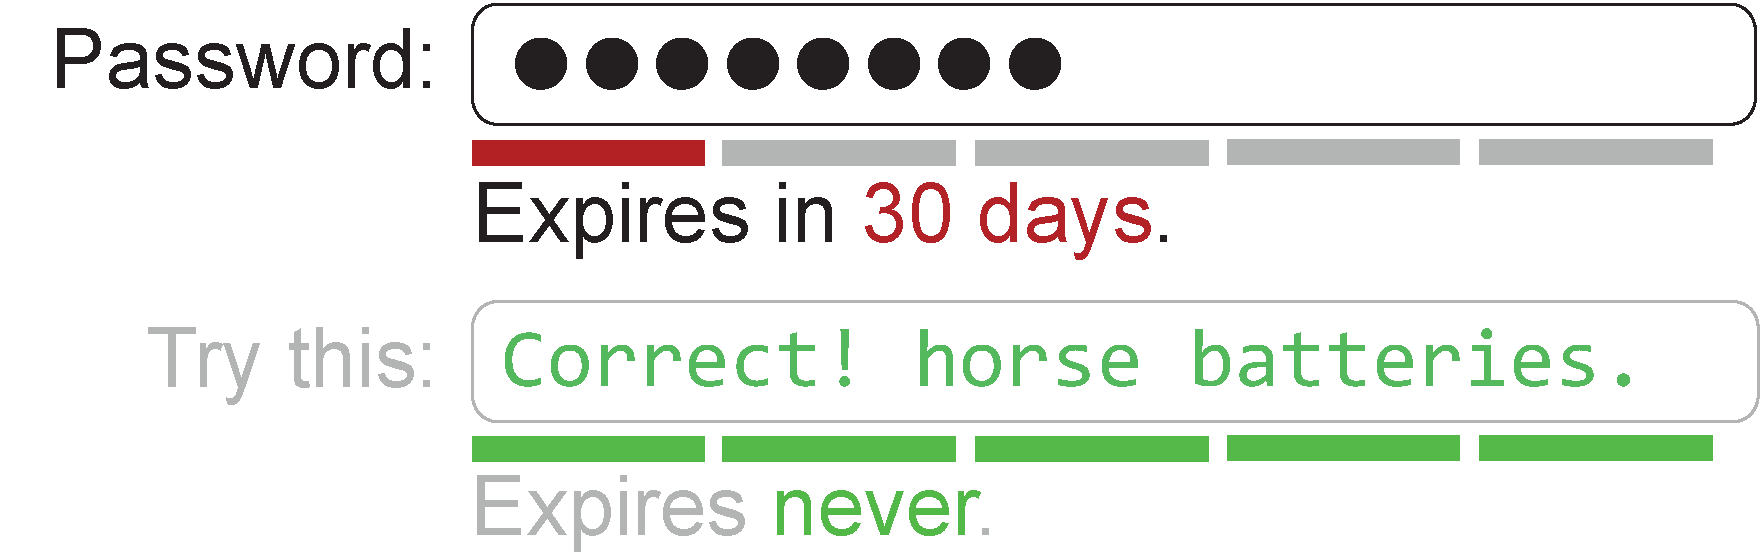
\includegraphics[width=0.5\linewidth]{figures/decoy/expire_mockup}
	\caption{\label{fig:decoy:expiremockup}Suggestion accompanied by a graspable benefit.}
\end{figure}

\section{Conclusion}
We set out to nudge users towards a password than is stronger than the first choice from their ``comfort zone''. From theories in behavioral economics we carefully derived a choice architecture that translates marketing strategies to ``password advertisement''. This direct translation, however, did not produce the envisioned decoy effects in our online study with 83 participants. Instead, we found that encouraging people through an easily achievable goal fostered a positive outcome: If participants saw that a passphrase containing no digits and symbols could be ``very strong'' they managed to create stronger passwords on average. We conclude that simplifying the sub-task to compare one's own performance to a suggested alternative is a key to successfully nudging users in this direction. To avoid that such nudges wear off over time, they should only be used in situations where the benefit of choosing a stronger password is graspable and evident to users. 

%TODO: pick up the requirements from chapter \ref{chap:feedback_modalities}

%Future Work
Although the decoy effect did not show, this does not mean it does not exist for passwords. It could simply mean that the direct adaptation of choice architectures in other fields is insufficient and needs more fine-tuning. In a different UI design, where the dimensions are more clearly framed for the users, the hypothesized preferential shift might be induced. A possible direction towards this is to step away from generating completely new passwords and instead nudge users towards a modified version that significantly increases strength. Ur \etal have already provided first positive results about suggesting password alterations. It would be interesting to find out if an additional alteration that is ``unattractive by design'' could boost adoption rates of the target suggestion. We see many opportunities to further explore persuasive password suggestions, especially if they remove usability pain points of trying to create a memorable yet strong secret. 

\vspace*{1cm}\noindent
\fbox{
	\hspace{1cm}
	\parbox[c][8cm]{0.7\linewidth}{
		\section*{Take Aways}
		\begin{itemize}[leftmargin=*]
			\item The decoy effect was \textbf{not} visible when participants received two suggestions. They proceeded with their own passwords. The most plausible explanation is that the benefits of the target over the decoy were too vague. 
			\item Demonstrating that strong passwords do not have to be overly complicated by suggesting and a passphrase made our participants select stronger passwords. Using feed-forward appears to encourage people to come up with a better secret. %However, this needs to be confirmed in another study. 
		\end{itemize}
	}
	\hspace{1cm}
}

